% this TeX file provides an awesome example of how TeX will make super 
% awesome tables, at the cost of your of what happens when you try to make a
% table that is very complicated.
% Originally turned in for Dr. Nico's Security Class
\documentclass[10.8pt]{article}

\usepackage{url}

% text shouldn't exceed 6 inch width and 8 inch height
\usepackage[a4paper, total={6in, 8in}, margin=0.8in]{geometry}

% makes it so that the first paragraph of every section is indented
\usepackage{indentfirst}

% For listing code
\usepackage{listings}

\usepackage{color}

% For lst entries (code)
\definecolor{mygreen}{rgb}{0,0.6,0}
\definecolor{mygray}{rgb}{0.5,0.5,0.5}
\definecolor{mymauve}{rgb}{0.58,0,0.82}

\lstset{ %
  backgroundcolor=\color{white},   % choose the background color
  basicstyle=\footnotesize,        % size of fonts used for the code
  breaklines=true,                 % automatic line breaking only at whitespace
  captionpos=b,                    % sets the caption-position to bottom
  commentstyle=\color{mygreen},    % comment style
  escapeinside={\%*}{*)},          % if you want to add LaTeX within your code
  keywordstyle=\color{blue},       % keyword style
  stringstyle=\color{mymauve},     % string literal style
  frame = single,
}
   

\usepackage{titlesec}


% math equation package, "fleqn" positions equations at a fixed indent from the left margin
% math equation leqno brings the numbering for equations to left side
\usepackage{amsmath}

\usepackage{parskip}
\setlength{\parskip}{.8em}

% Set the indent to zero for the whole document
\setlength\parindent{0pt}





% For graphics/images
\usepackage{graphicx}



% For captions under images
\usepackage{caption}

% float package for image alignment
\usepackage{float}
% images are in the directory images/
\graphicspath{ {images/} }

% \usepackage{pagecolor}% With option pagecolor={somecolor or none}
% \definecolor{ultramarine}{RGB}{253,255,244} 

% degree symbol: \degree
\usepackage{gensymb}



\begin{document}

% \pagecolor{ultramarine}



\begingroup  
\vspace{2em}
  \centering
  \LARGE \textbf{Internal Positioning System (IPS) Application For Android\\[0.4em]}
  \large Andre Bododea \\[0.2em]
  \large s1350924 \par

\endgroup


\vspace{1em}

\section*{Part 1: User Guide}

The purpose of this paper is to discuss an Indoor Positioning System (IPS) application designed for Android. GPS cannot function accurately within a building, therefore there is a strong need for IPS to take over tracking the user from the GPS once he steps within a building. This application attempts to solve this problem by using RSS scans from WiFi access points. The user must first train the floor plan of the building he/she is currently within. The RSS values for positions on the map are recorded in persistent memory via a database as the user walks around performing the training. Once enough points are collected, the user can then use the application in order to track themselves as they walk around the building.

\vspace{1em}

\begin{figure}[H]
    \centering
    \begin{minipage}[b]{.3\textwidth} 
        \centering  
        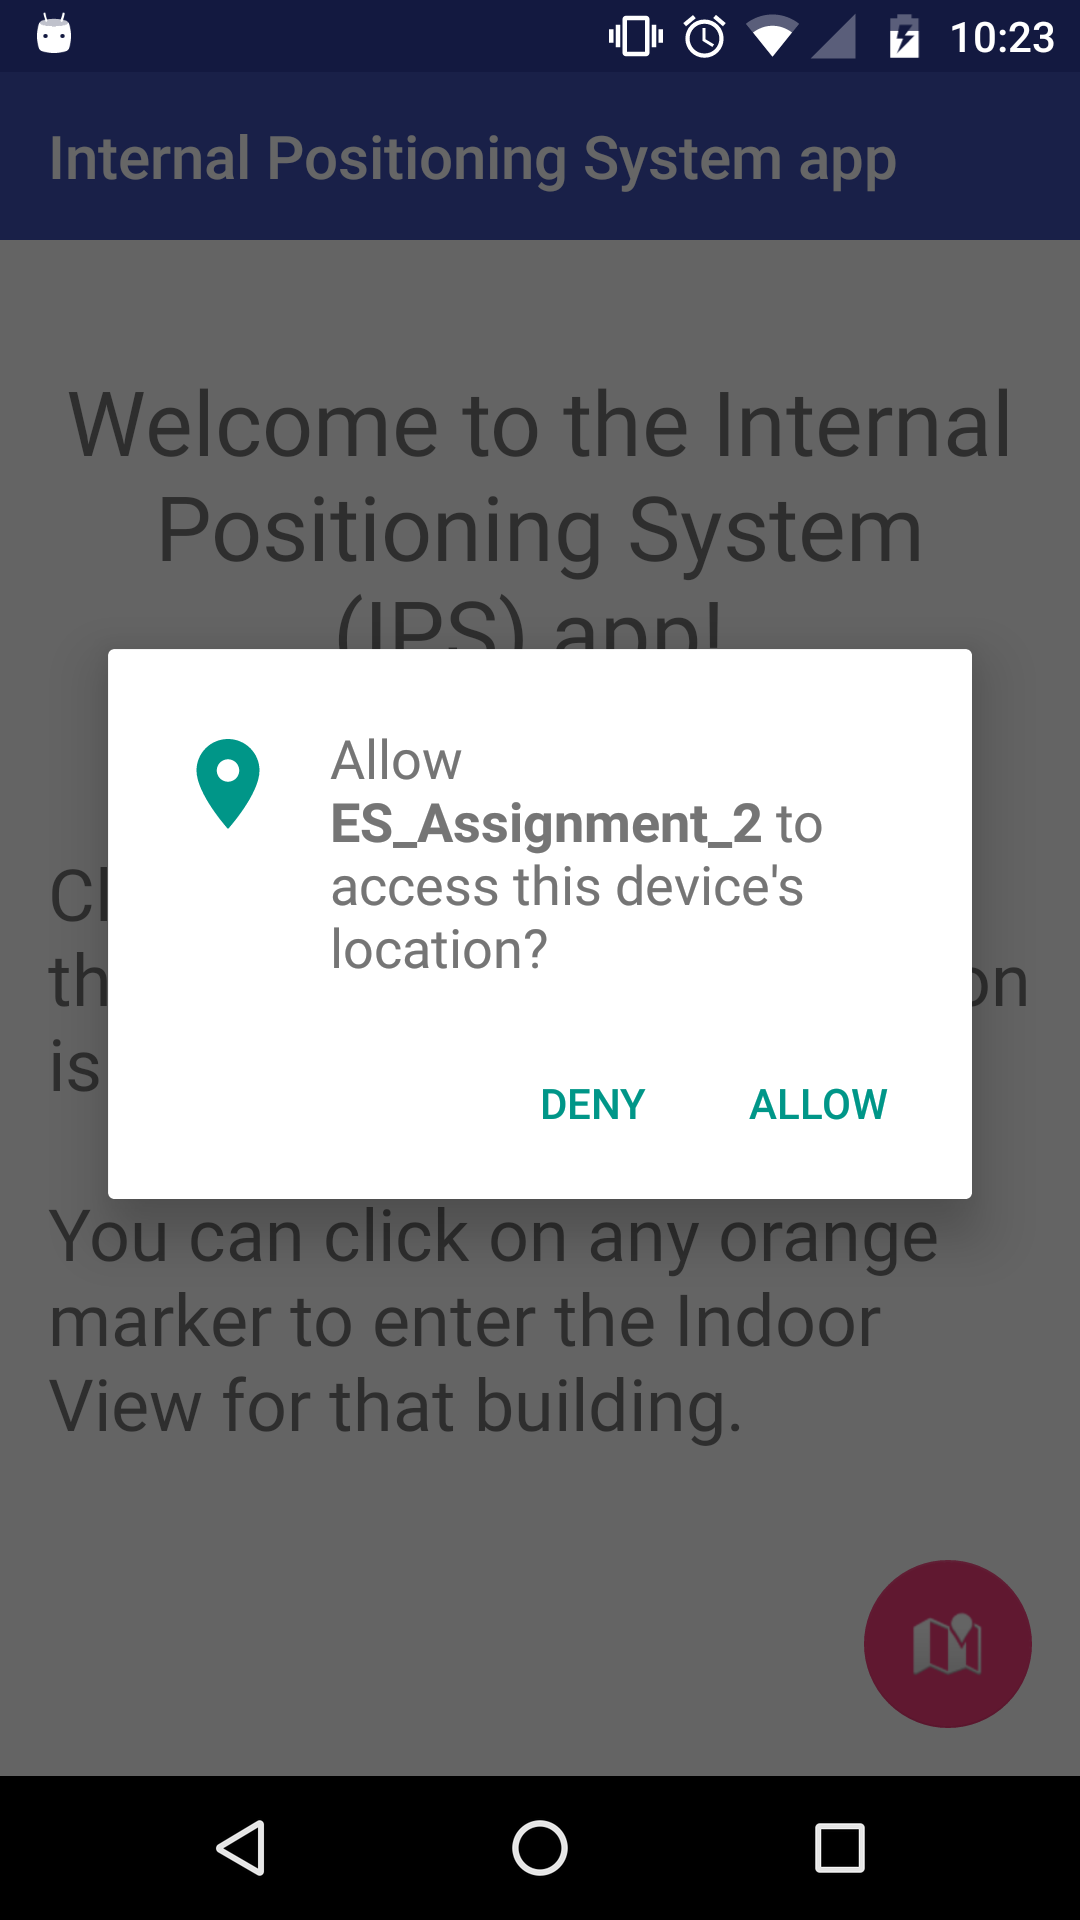
\includegraphics[scale=1.2, width=\linewidth]{pic0.png}     
        \caption{Requesting user permissions}  
        \label{fig:1}
    \end{minipage}    
    \hfill
    \begin{minipage}[b]{.3\textwidth}  
        \centering  
        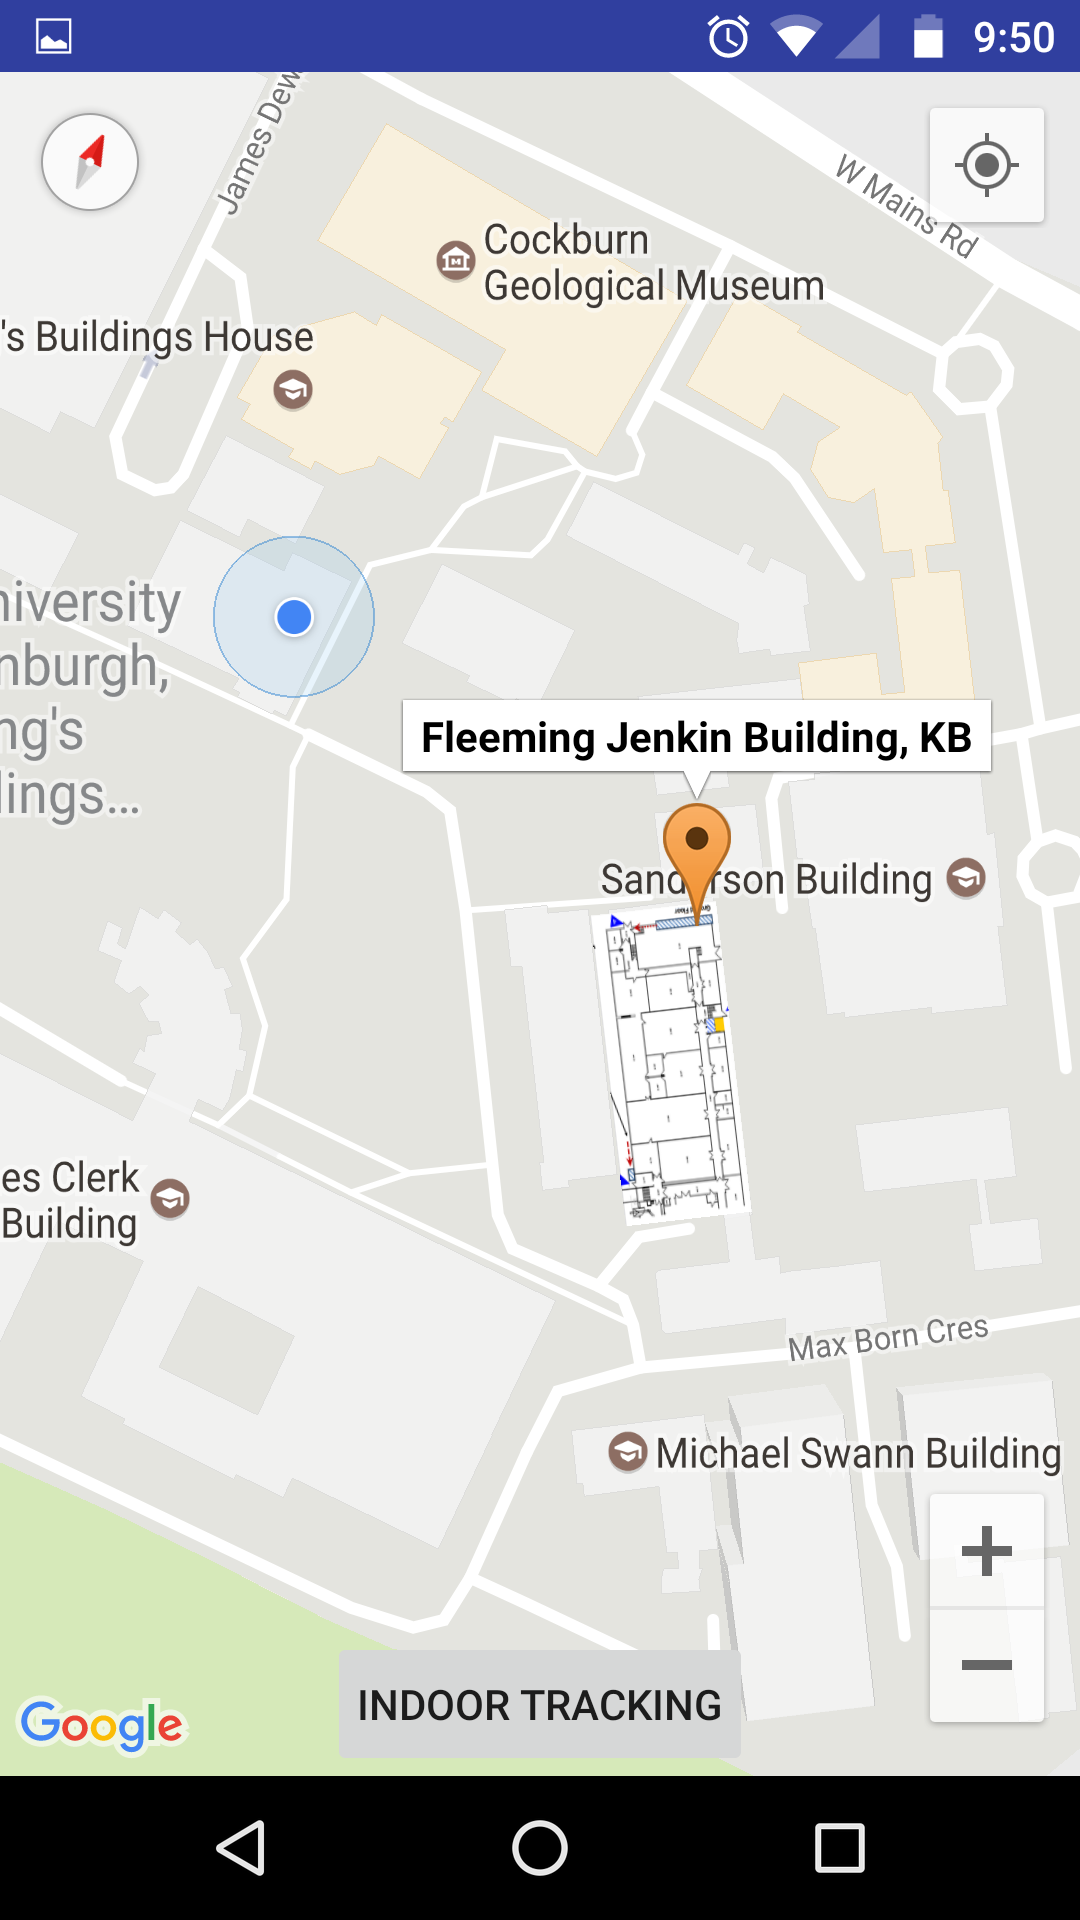
\includegraphics[scale=1.2, width=\linewidth]{pic1.png}  
        \caption{Current location on Google map view}  
    \end{minipage} 
    \hfill
    \begin{minipage}[b]{.3\textwidth}  
        \centering  
        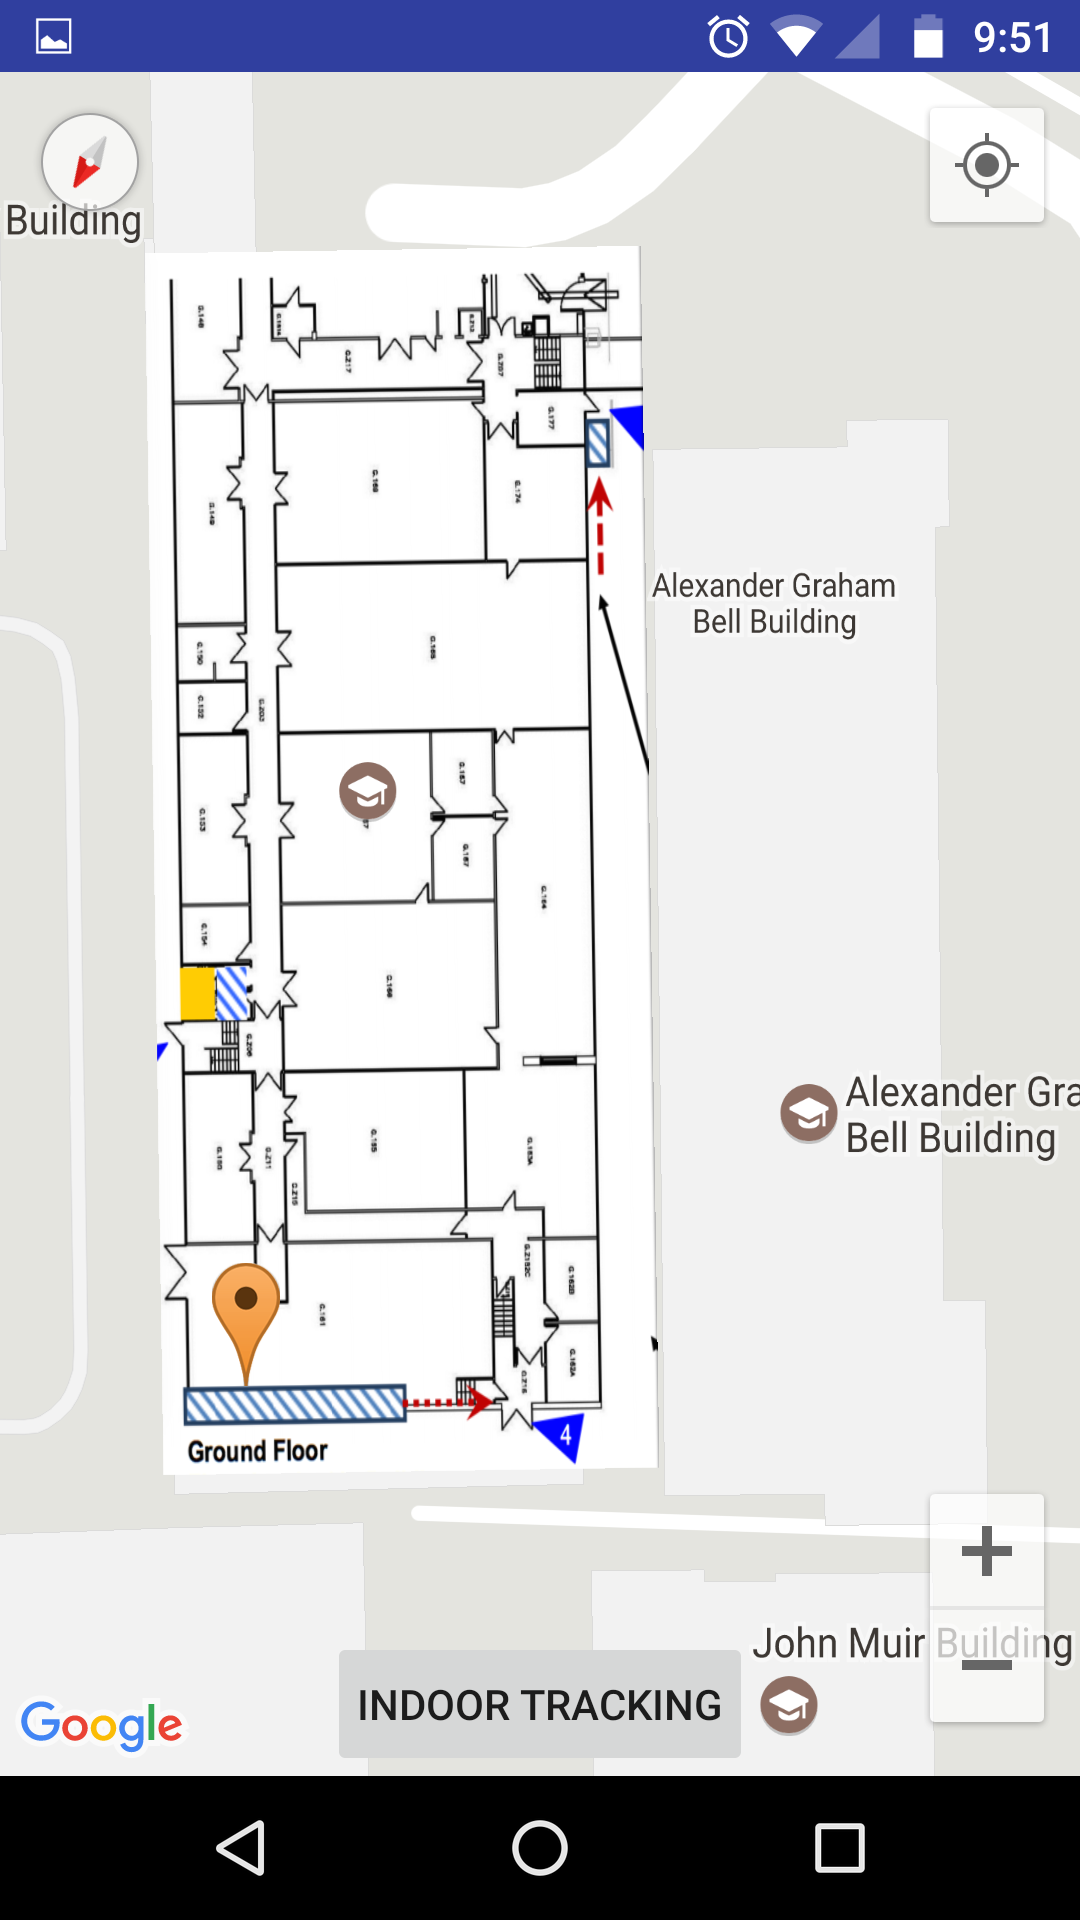
\includegraphics[scale=1.2, width=\linewidth]{pic2.png}  
        \caption{Building with floor plan overlayed}  
    \end{minipage}  
\end{figure}

Immediately after installation, as the user opens the app a prompt opens asking them to enable location permissions (\textbf{Fig 1}). This permission is integral to the app's ability to function, as without it we cannot complete our scans. If the user does not accept, the app will not be launched. After this, the user is presented with a standard Google map. The user can press the location button in the top right-hand corner to zoom in on his/her current location (\textbf{Fig 2}). If this location is near a building with a floor plan overlayed, there will also be an option to click on an orange marker to enter the \textit{indoor view} (\textbf{Fig 3}). Once they have reached this indoor view, training instructions for the floor plan for that building will be shown. The user is told to draw their desired path that they will then follow in order to complete the training of the database.



\begin{figure}[H]
    \centering
    \begin{minipage}[b]{.3\textwidth} 
        \centering  
        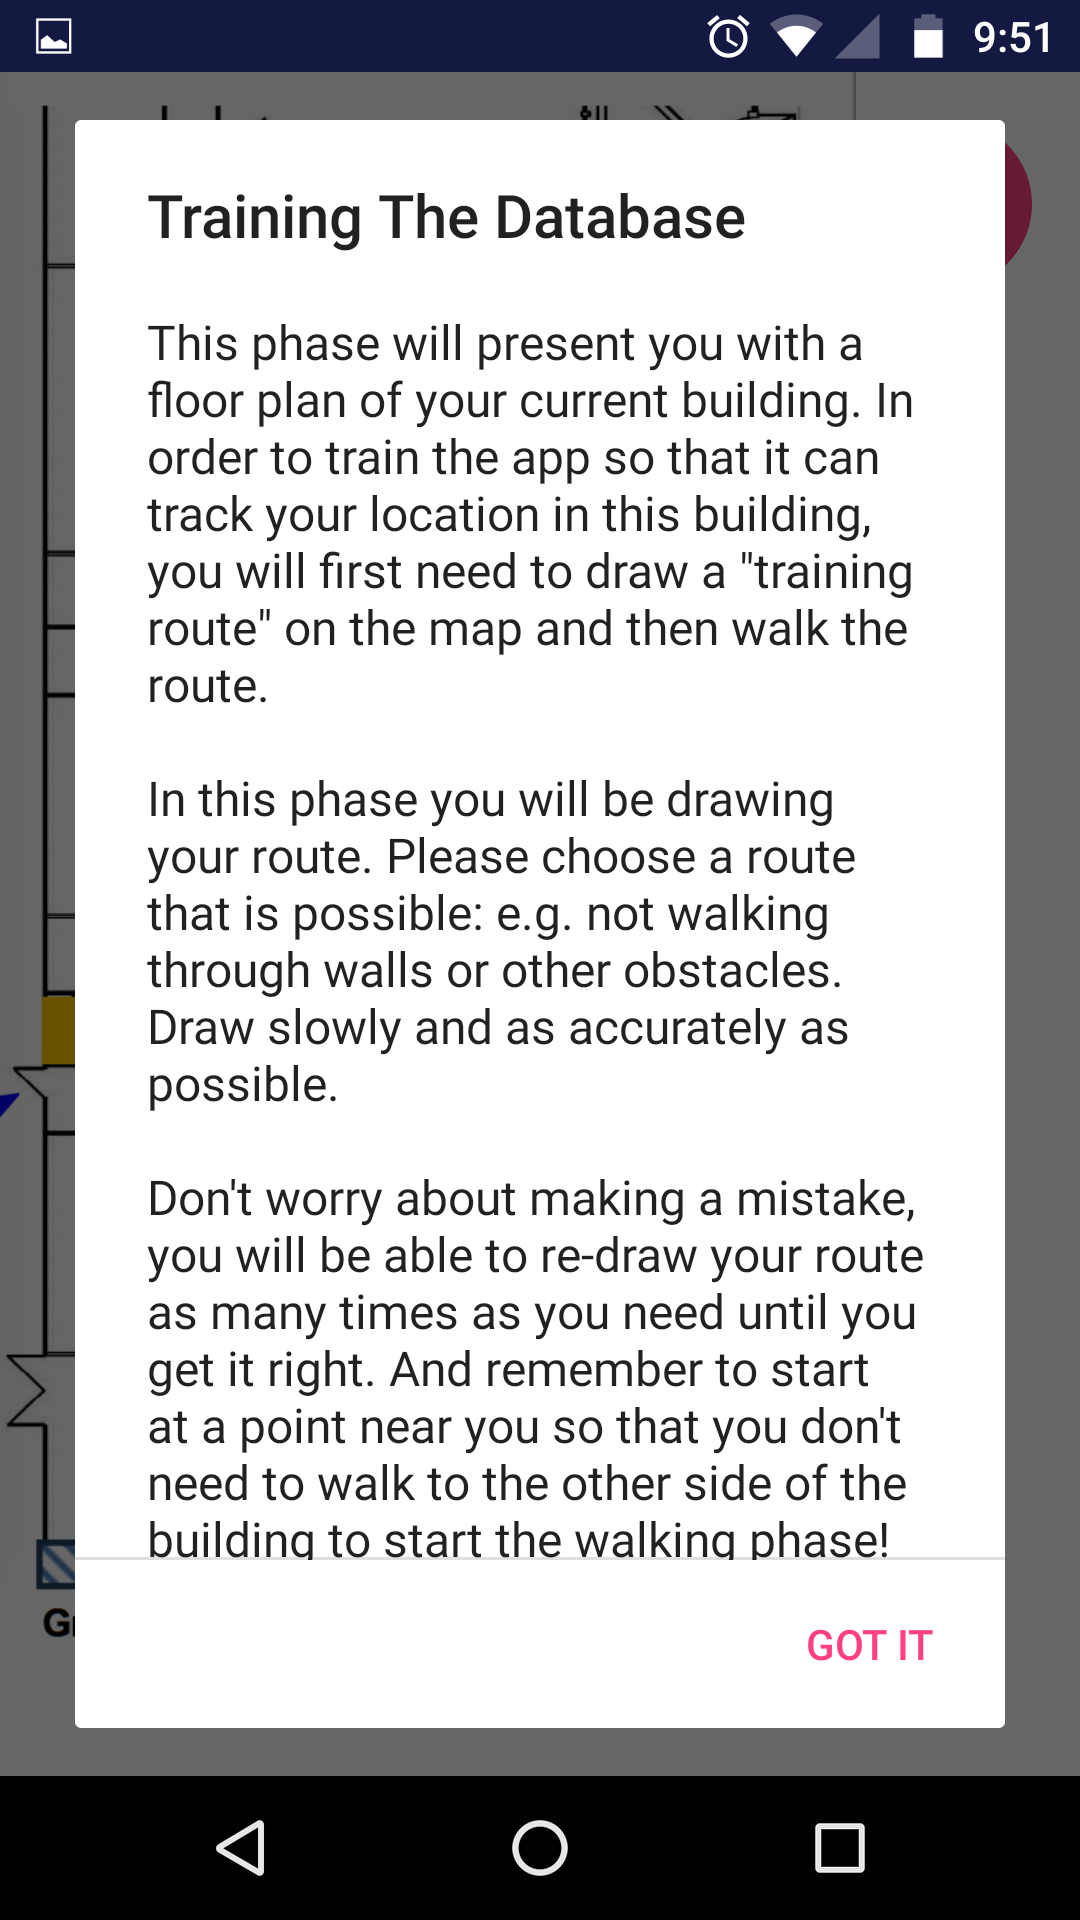
\includegraphics[scale=1.2, width=\linewidth]{pic3.png}     
        \caption{Training instructions once in indoor view}  
        \label{fig:1}
    \end{minipage}    
    \hfill
    \begin{minipage}[b]{.3\textwidth}  
        \centering  
        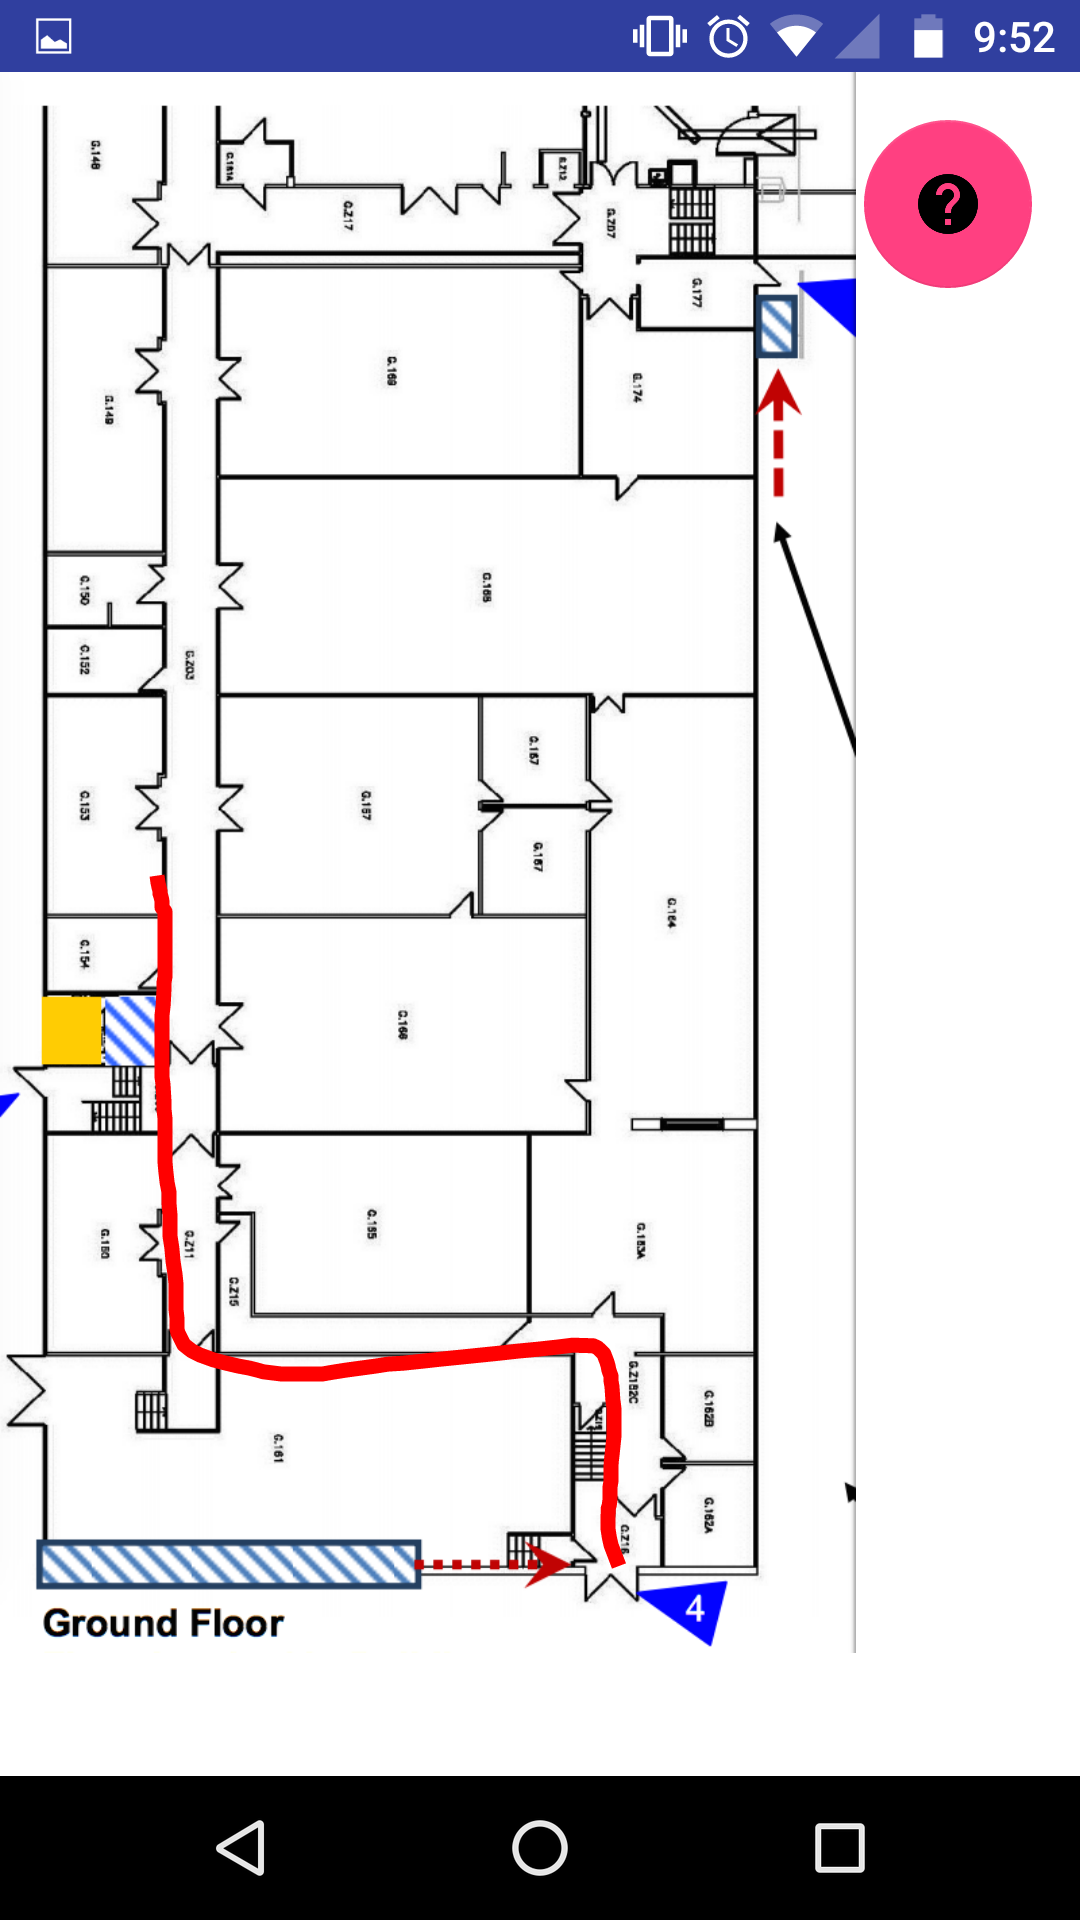
\includegraphics[scale=1.2, width=\linewidth]{pic4.png}  
        \caption{User drawing their chosen training path}  
    \end{minipage} 
    \hfill
    \begin{minipage}[b]{.3\textwidth}  
        \centering  
        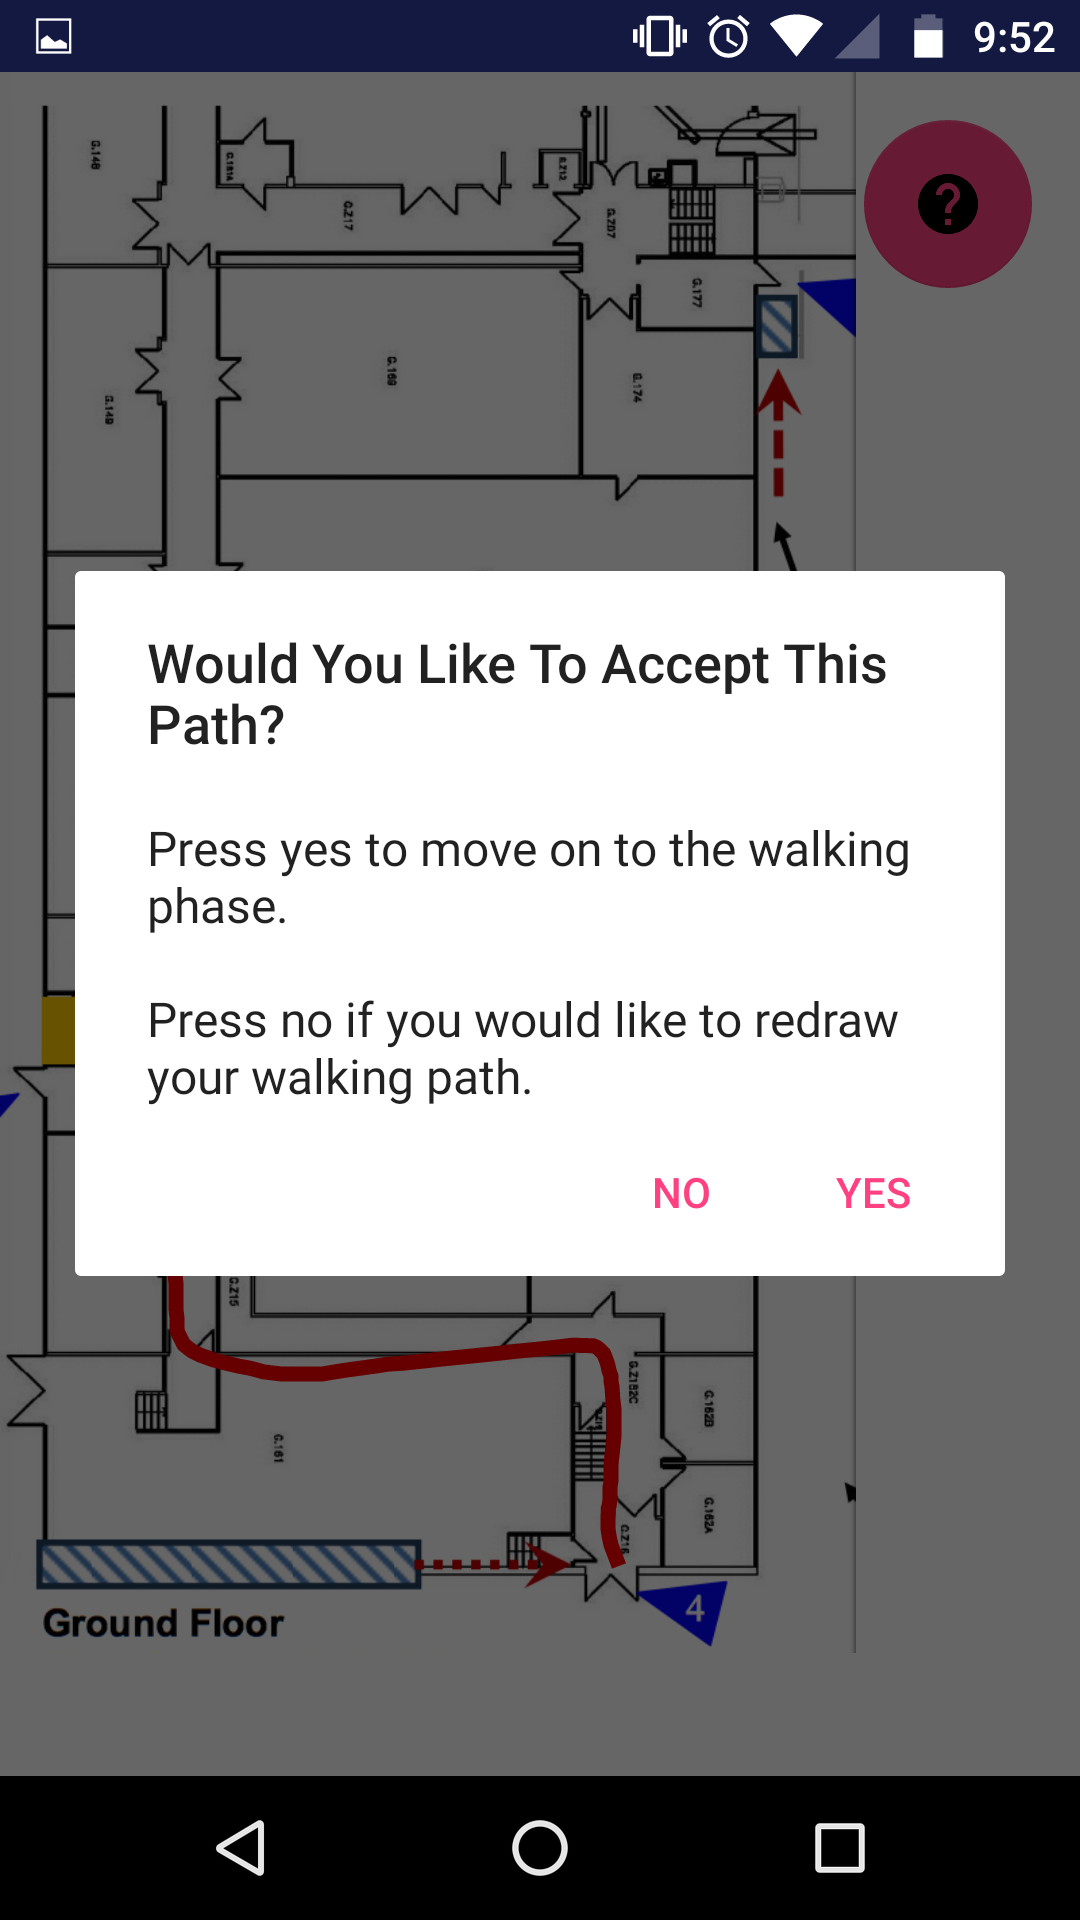
\includegraphics[scale=1.2, width=\linewidth]{pic5.png}  
        \caption{Prompt to accept the path}  
    \end{minipage}  
\end{figure}

Once the user has drawn a path (\textbf{Fig 5}), he/she must then follow this path as an animated green dot walks them through the path (\textbf{Fig 8}). They must try to follow the green dot as closely as possible in order to accurately train the data set.

\vspace{1em}

\begin{figure}[H]
    \centering
    \begin{minipage}[b]{.3\textwidth} 
        \centering  
        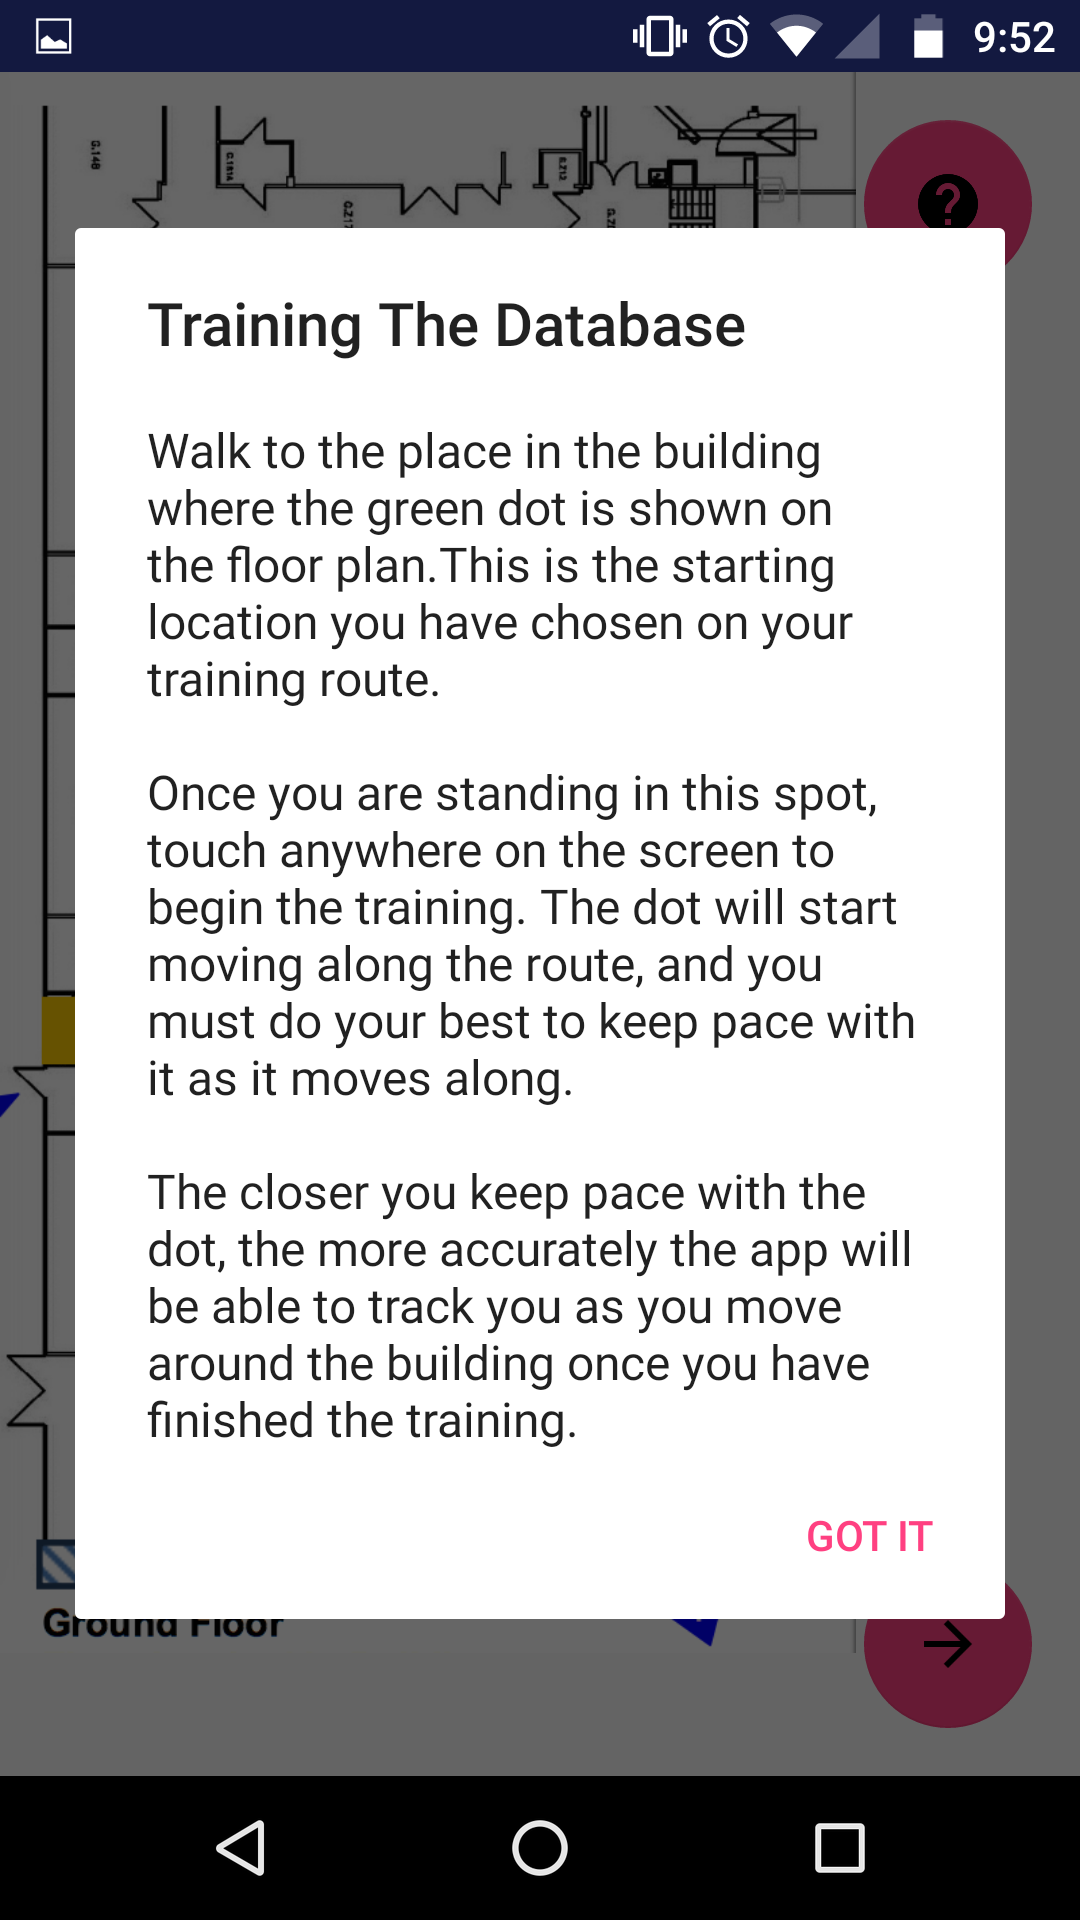
\includegraphics[scale=1.2, width=\linewidth]{pic6.png}     
        \caption{Training instructions for following the training animation}  
        \label{fig:1}
    \end{minipage}    
    \hfill
    \begin{minipage}[b]{.3\textwidth}  
        \centering  
        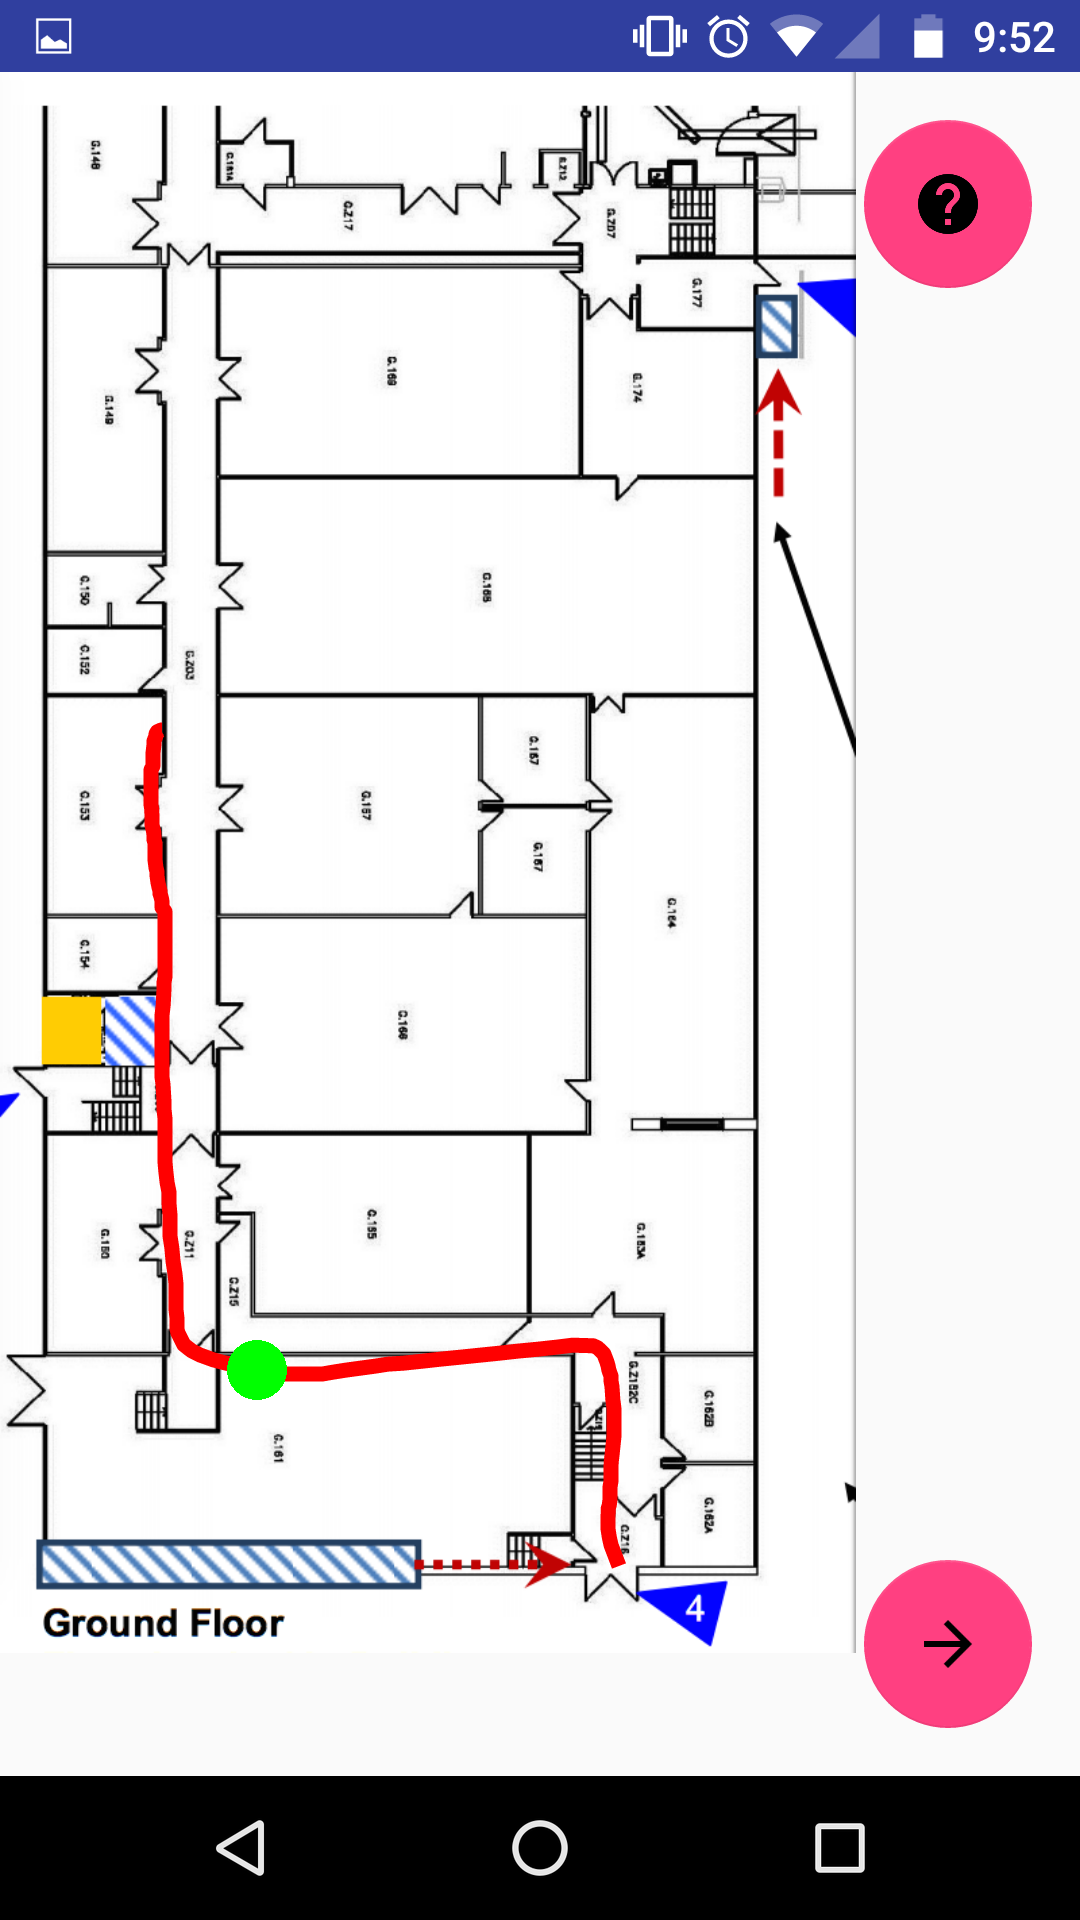
\includegraphics[scale=1.2, width=\linewidth]{pic8.png}  
        \caption{Training animation in progress, user is walking path}  
    \end{minipage} 
    \hfill
    \begin{minipage}[b]{.3\textwidth}  
        \centering  
        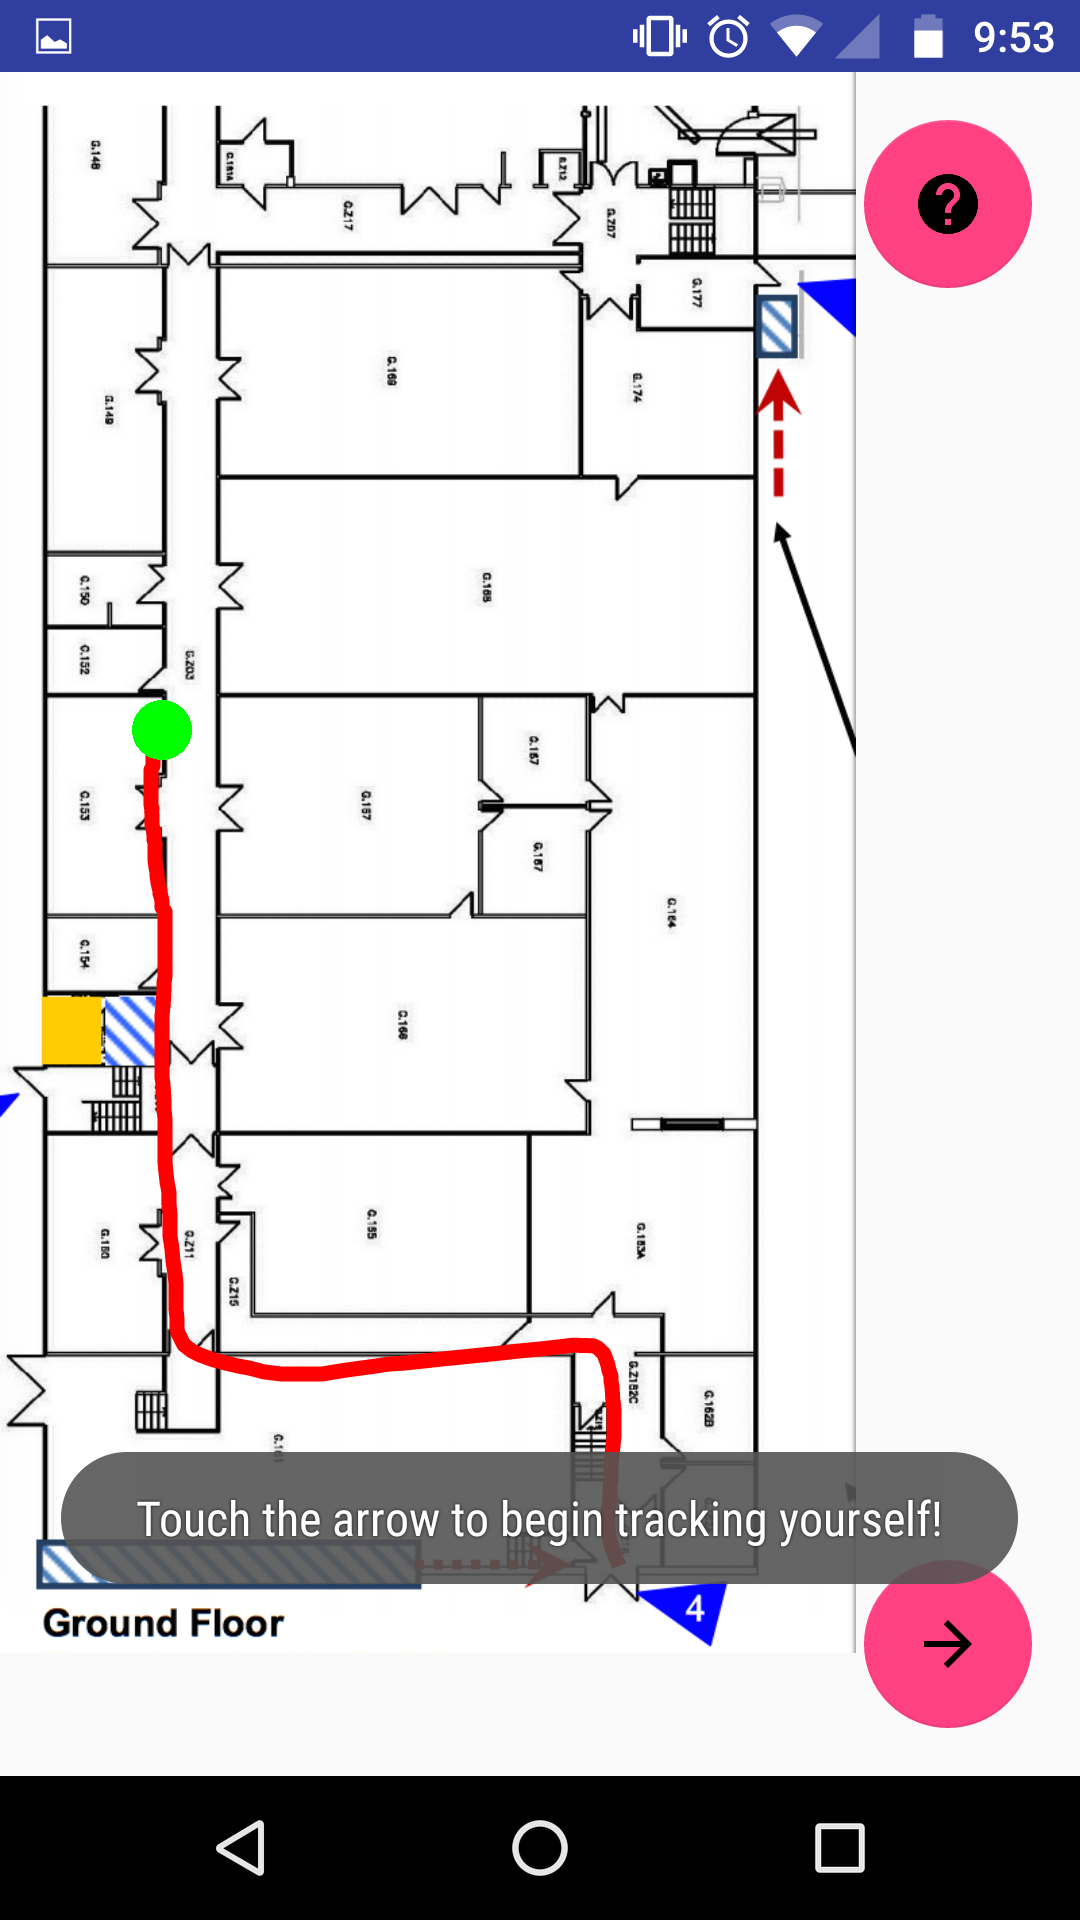
\includegraphics[scale=1.2, width=\linewidth]{pic9.png}  
        \caption{End of path reached, training is now finished}  
    \end{minipage}  
\end{figure}

Once the user has drawn a path then physically walked that path in order to train the database on a set of scan points, he/she can now use the floor plan to track his/her position in the building \textit{for the region trained in their path} (\textbf{Fig 10} \& \textbf{11}). The app will attempt to find the closest trained point from the database, and match it to the user's current position on the map via WiFi scans.

\begin{figure}[H]
    \centering
    \begin{minipage}[b]{.3\textwidth} 
        \centering  
        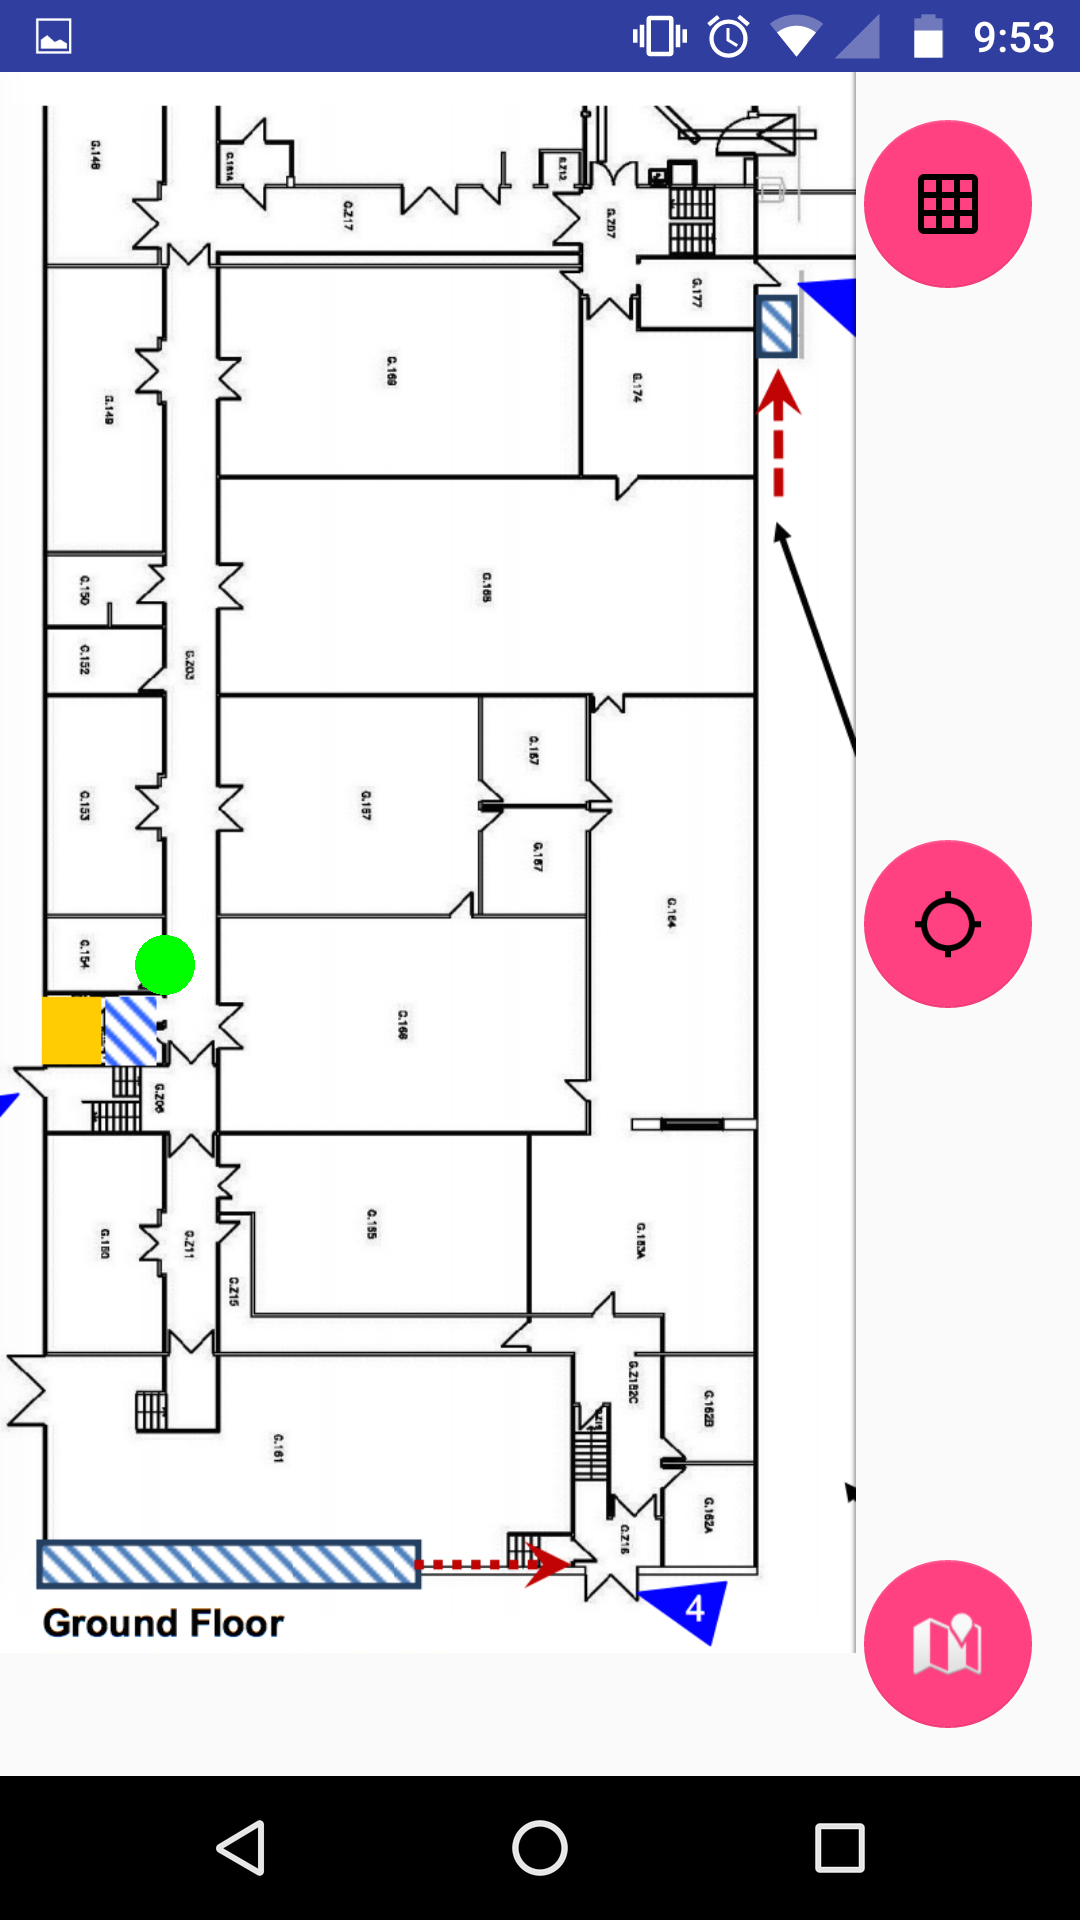
\includegraphics[scale=1.2, width=\linewidth]{pic10.png}     
        \caption{Tracking the user's position on the floor plan while moving around building}  
        \label{fig:1}
    \end{minipage}    
    \hfill
    \begin{minipage}[b]{.3\textwidth}  
        \centering  
        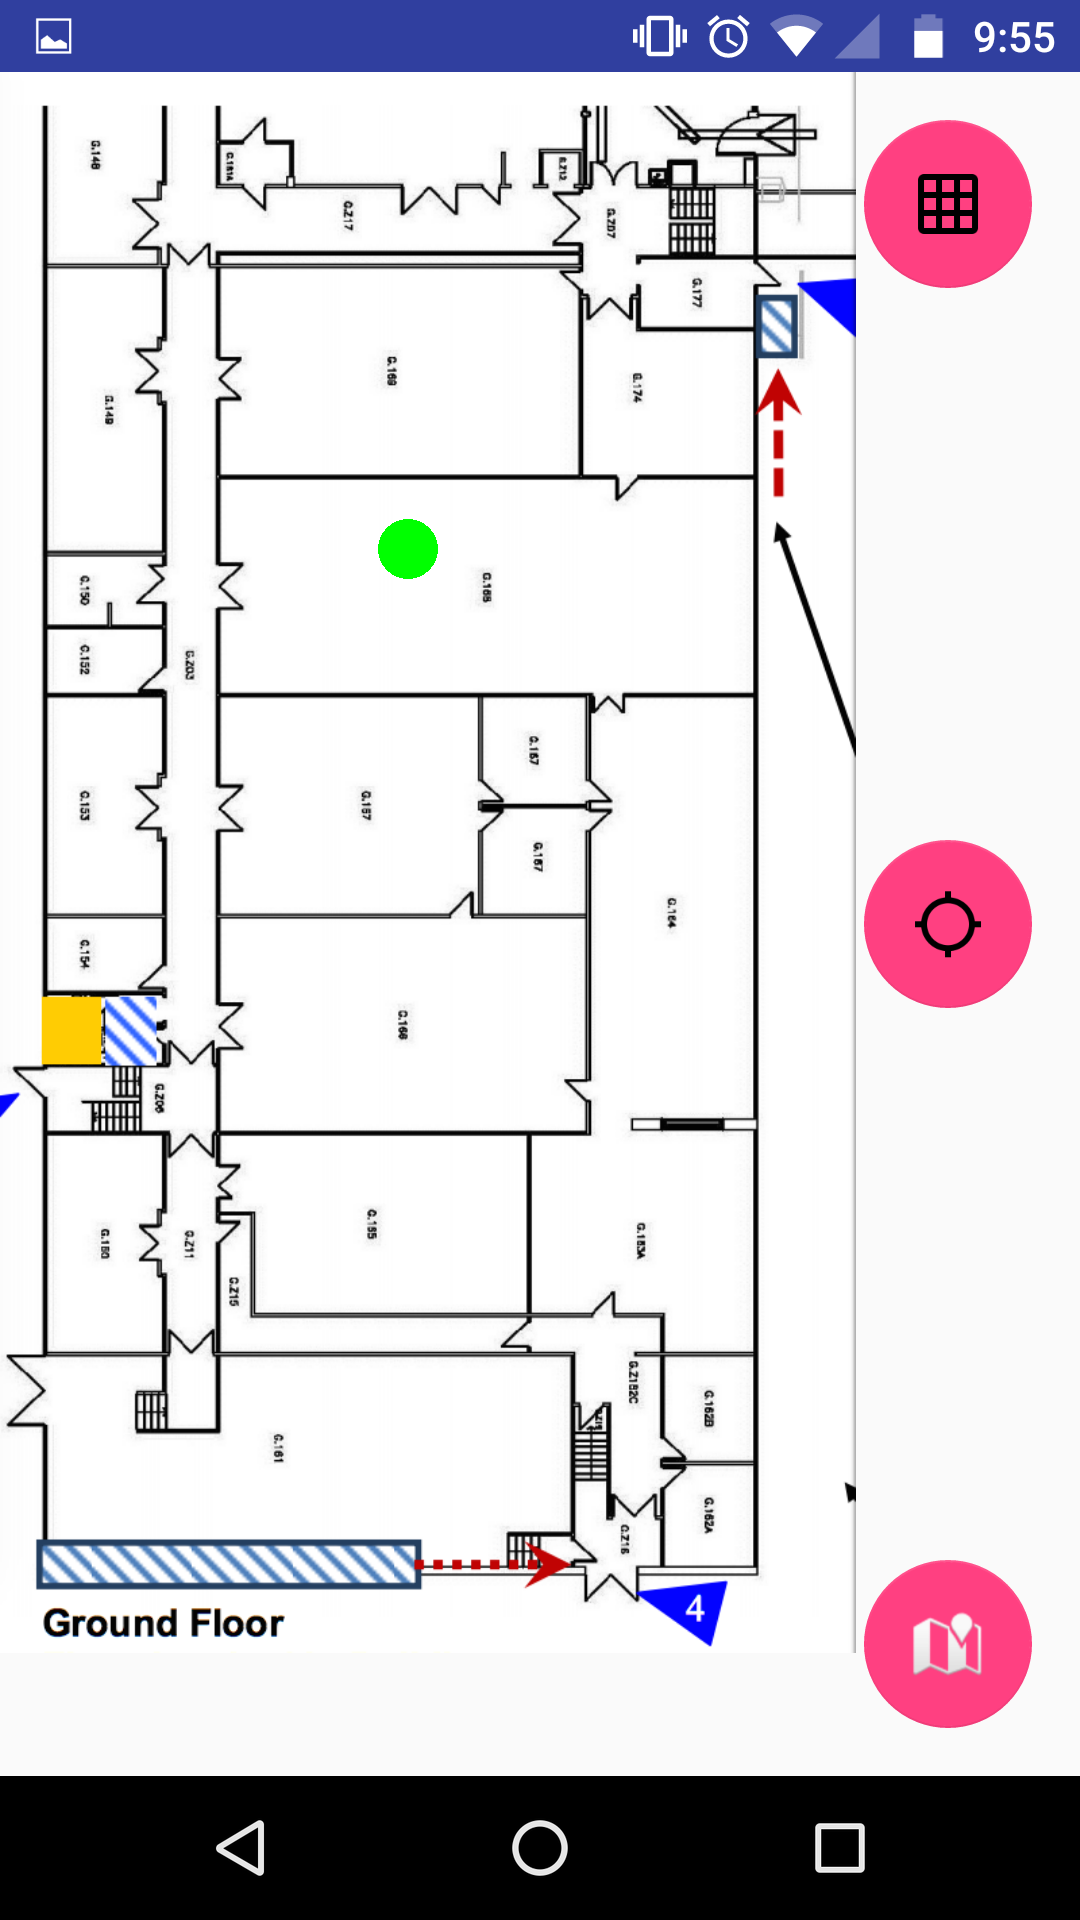
\includegraphics[scale=1.2, width=\linewidth]{pic13.png}  
        \caption{After another few sets of trainings, the user can have a wider range on the map}  
    \end{minipage} 
    \hfill
    \begin{minipage}[b]{.3\textwidth}  
        \centering  
        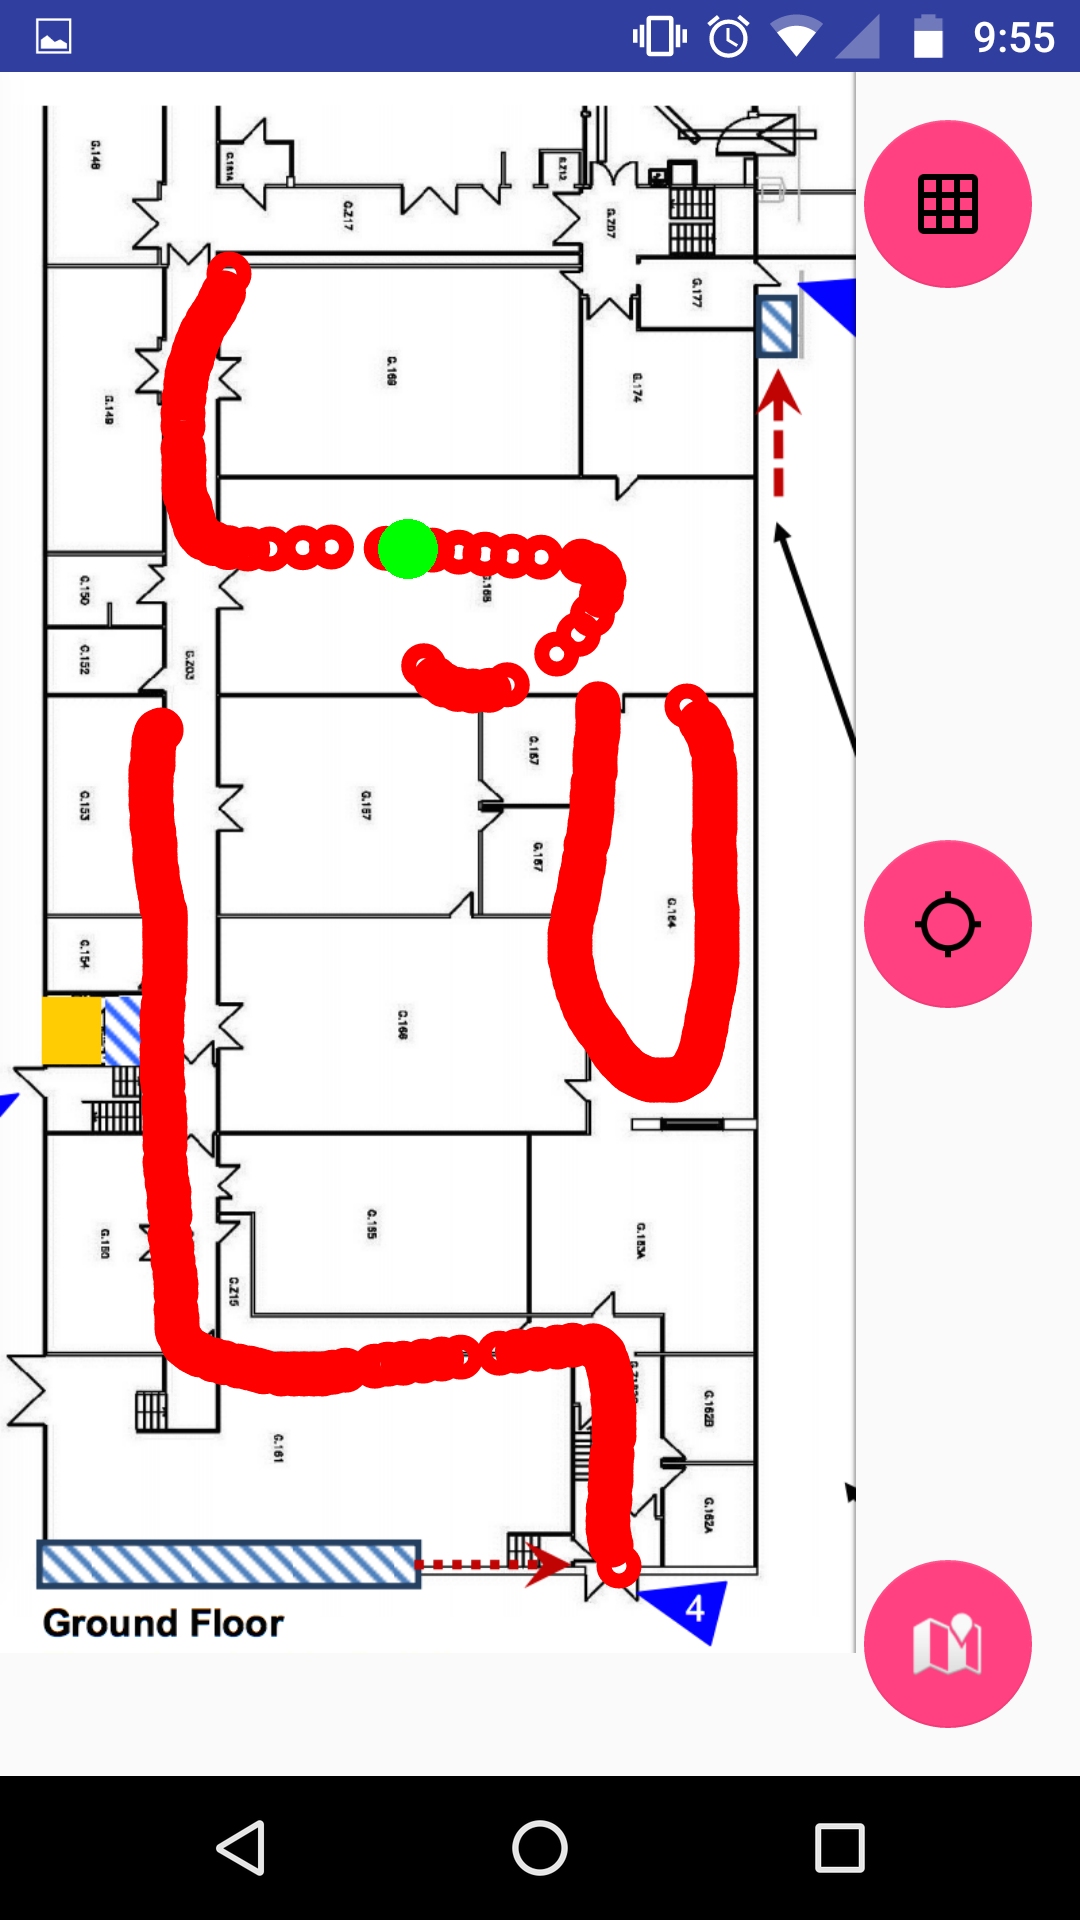
\includegraphics[scale=1.2, width=\linewidth]{pic14.png}  
        \caption{"Grid" button shows all previously recorded paths in the database}  
    \end{minipage}  
\end{figure}

The user can record as many different paths as they want, and use the "grid" button in the upper right-hand corner to view all the paths already trained (\textbf{Fig 12}). This gives them an idea of what parts of the building tracking is available and what parts have yet to be trained. The button with the map icon in the lower right-hand corner takes us back to the map view from \textbf{Figs 2} \& \textbf{3}.

With this simple, easy to use interface, along with an animated training system that allow users to train any building quickly and flexibly, this app requires no technical know-how and makes indoor positioning simple and accessible for casual users.


\section*{Part 2: Developer Guide}

This application was designed to be \textit{highly modular}. Each screen has its own Activity class, and important values are passed via Intent to the next Activity class in the call-order. 

Techniques for localisation using radio signal can take advantage of numerous technologies - Bluetooth, WiFi, and cellular signals just to name a few \cite{shchekotov2014indoor}. Localisation via WiFi was chosen for the simple reason that WiFi hotspots are available in most public buildings, and no additional infrastructure setup is needed to work with them \cite{kashevnik2012comparative}.

This app was designed to take advantage of WiFi access points, or more specifically RSS scans. The concept of triangulating via RSSI scans is certainly not a new or particularly complex one. It was explored at length as early as 2004 by Kaemarungsi et all  \cite{kaemarungsi2004modeling}, however advances in RSSI localisation algorithms continue to be made \cite{alsehly2010improving,oguejiofor2013outdoor} and continue to show it to be the most powerful and flexible tool for IPS available today.


\subsection*{Implementation: Sensors and APIs }


\subsubsection*{Google Maps API}

In order to be able to have such a beautiful and responsive map interface, we have implemented our outdoor map using Google Maps Android API \cite{google_maps_api}. Along with being a great app that allows tonnes of features such as pins and floor plan overlay (\textbf{Figs 2} \& \textbf{3}), using the Google Maps API   allows the added bonus of user being familiar with the layout and use of the map.

\subsubsection*{WifiManager}

Once we are in our \textit{inside view}, the most important tool we have is the WifiManager. This API allows us to manage all aspects of Wifi connectivity

The most important use for WifiManager in this app is getting nearby access point addresses and their corresponding signal strengths. The code below shows how we use the WifiManager to get these values for the location where the user is currently standing.    

\vspace{1em}      

\begin{lstlisting}[language=java,caption=Get BSSID values and corresponding signal strengths at current location via the WifiManager API]
WifiManager wifiManager  = (WifiManager) context.getSystemService(Context.WIFI_SERVICE);
List<ScanResult> wifiList = wifiManager.getScanResults();

ArrayList<String> networkAddresses = new ArrayList<String>();
ArrayList<Integer> signalStrengths = new ArrayList<Integer>();

// Add the BSSIDs and corresponding signal strengths to the lists
for (ScanResult scanResult : wifiList) {
    networkAddresses.add(scanResult.BSSID);
    signalStrengths.add(Math.abs(scanResult.level));
}
\end{lstlisting}

Once we have these values, they must be stored somewhere. In order to be used over the lifetime of the app, and not just for the current session, the data storage must be \textit{persistent}. The best form of persistent storage for us in a small application situation such as this one is a database.

\section*{Database}

Android ships with a powerful API for interfacing with SQL databases, called SQLite \cite{sqlite_api}. We design a database to store the values found from the WifiManager, stored for each point on the map. This database must store the point on the floor plan, denoted by an x-y coordinate pair. It must also store all the BSSIDs and corresponding signal strengths at that point on the floor plan.

\vspace{1em}

\begin{table}[H]
\centering
\label{my-label}
\begin{tabular}{|c|c|c|c|c|}  \hline
\textbf{PointID} & \textbf{xCoord} & \textbf{yCoord} & \textbf{BSSID} & \textbf{SignalStrength} \\ \hline  \hline
1 & 1003.789018 & 7314.123744 &  00:08:C7:1B:8C:02 & 79 \\ \hline 
1 & 1003.789018 & 7314.123744 & 20:29:B1:1A:5A:03  & 86 \\ \hline
1 & 1003.789018 & 7314.123744 & 02:28:A1:1A:22:31  & 61 \\ \hline
2 & 2991.345891 & 3423.812379 & 12:08:C7:1C:8B:02   & 64 \\ \hline
2 & 2991.345891 & 3423.812379 &  20:29:B1:1A:5A:01  & 72 \\ \hline
3 & 7237.345891 & 1234.567891 & 21:61:C2:8B:5A:B1   & 40 \\ \hline
. & . & . & . & . \\ \hline
\end{tabular}
\caption{Format of our SQL table for storing coordinates, BSSIDs, and SignalStrengths}
\end{table}

Each x-y point is associated with a unique PointID. This ensures no duplicates are chosen in querying the database when we are getting the nearest point based on the BSSID values. At each training point along the training route (the animation that the user is meant to walk along with), we query the WifiManager for all available BSSIDs and their corresponding signal strengths. These values are then stored in a table such as the one above. We can then query the table at a time when we need to access these data points, such as finding the nearest recorded data point to the user's position as in \textbf{Figs 10} \& \textbf{11}.

\section*{Finding The Nearest Point: K-nearest Neighbours}

We have training data stored in the database as discussed in the previous section, however we still have not discussed how we access this data and how we use it when predicting the user's nearest position on the map via RSSI signal strength. We use a modified version of the popular k-nearest neighbours method to do this.

We begin by getting the BSSIDs and signal strengths of our current location as in Listing 1 above. Then we use these values, and cycle through the database using SQL commands to extract the entries with matching BSSIDs. Once we have extracted these entries we simply extract the corresponding signal strength, and compute the Euclidian distance between that signal strength and the strength at the current position. 

By doing this over the entire set of points in the database, we can find the entry with the lowest mean distance between its signal strengths and the current signal strength across all BSSIDs. This point is considered the nearest point, and we simply use a query to extract the x and y values of the coordinates and then subsequently plot these values as a green dot on the floor plan (seen in \textbf{Figs 10} \& \textbf{11})


\section*{Conclusion}

Overall, this application is robust to changing environments as WiFi is so widespread a technology. Further steps could involve inclusion of other data - EMF (Magnetic Field), Radio Frequency, Bluetooth. An interesting further step would be literally that - including a step counter to not only assist with accurate pacing of the user with the training animation, but to eventually replace the animation with a self-training step counter based implementation that trains as you walk around the building. All of these additional technologies will be considered for inclusion in version 2 of this application. As a first release, however, this IPS application can serve as a gentle introduction for the average user to IPS through its easy to use UI. Animations guide the user through the process making it simple and even fun to take part in using IPS.


\vspace{\baselineskip}

\bibliographystyle{unsrt}
\bibliography{es2}


\end{document}


